%%%%%%%%%%%%%%%%%%%%%%%%%%%%%%%%%%%%%%%%
% datoteka diploma.tex
%
% vzorčna datoteka za pisanje diplomskega dela v formatu LaTeX
% na UL Fakulteti za matematiko in fiziko
%
% vkup spravil Gašper Fijavž, december 2010
% množica popravkov v januarju, februarju marcu 2011
% verzijo 29. marec 2011 za FMF 19.9.2013 prilagodil Rok Mihevc
%%%%%%%%%%%%%%%%%%%%%%%%%%%%%%%%%%%%%%%%

\documentclass[a4paper, oneside, 12pt]{book}

\usepackage[utf8]{inputenc}   % omogoča uporabo slovenskih črk kodiranih v formatu UTF-8 
\usepackage[slovene,english]{babel}    % naloži, med drugim, slovenske delilne vzorce
\usepackage[pdftex]{graphicx}  % omogoča vlaganje slik različnih formatov 
\usepackage{fancyhdr}          % poskrbi, na primer, za glave strani
\usepackage{amssymb}           % dodatni simboli
\usepackage{amsmath}           % eqref, npr.
\usepackage{verbatim}           % \begin{comment} in \end{comment}
\usepackage{float}

\renewcommand{\baselinestretch}{1.3} % ustrezen razmik med vrsticami

%oznake strani

\renewcommand{\chaptermark}[1]%
{\markboth{\MakeUppercase{\thechapter.\ #1}}{}} \renewcommand{\sectionmark}[1]%
{\markright{\MakeUppercase{\thesection.\ #1}}} \renewcommand{\headrulewidth}{0.5pt} \renewcommand{\footrulewidth}{0pt} 
\fancyhf{}
\fancyhead[LE,RO]{\sl \thepage} \fancyhead[LO]{\sl \rightmark} \fancyhead[RE]{\sl \leftmark}

\newcommand{\BibTeX}{{\sc Bib}\TeX}

\newcommand{\autfont}{\Large}
\newcommand{\titfont}{\LARGE\bf}
\newcommand{\clearemptydoublepage}{\newpage{\pagestyle{empty}\cleardoublepage}}
\setcounter{tocdepth}{1}	      % globina kazala

% konstrukti
\newtheorem{izrek}{Izrek}[chapter]
\newtheorem{trditev}{Trditev}[izrek]
\newenvironment{dokaz}{\emph{Dokaz.}\ }{\hspace{\fill}{$\Box$}}

\begin{document}
\selectlanguage{slovene}
\frontmatter
\setcounter{page}{1} %
\renewcommand{\thepage}{}       % preprecimo težave s številkami strani v kazalu 

\begin{comment}

%naslovnica
\thispagestyle{empty}%
\begin{center}
  {\large\sc Univerza v Ljubljani\\%
    Fakulteta za Matematiko in Fiziko\\%
    Oddelek za Fiziko\\%
  Univerzitetni študij, naravoslovna smer}%
  \vskip 10em%
  {\autfont Rok Mihevc \par}%
  {\titfont Kraške vrtače Dinarskega krasa \par}%
  {\vskip 2em \textsc{DIPLOMSKO DELO}\par}%
  \vfill\null%
  {\large \textsc{Mentor}: prof.\ dr.  Rudolf Podgornik\par}%
%  {\large \textsc{Somentor}:  izr.\ prof.\ dr. \par}%
  {\vskip 2em \large Ljubljana, 2013 \par}%
\end{center}
% prazna stran
\clearemptydoublepage


% prazna stran
\clearemptydoublepage

%%%%%%%%%%%%%%%%%%%%%%%%%%%%%%%%%%%%%%%%
% izjava o avtorstvu
\vspace*{1cm}
\begin{center} 
  {\Large \textbf{\sc Izjava o avtorstvu diplomskega dela}}
\end{center}

\vspace{1cm}
\noindent Spodaj podpisani Rok Mihevc,
z vpisno številko \textbf{28030017}, sem avtor  diplomskega dela z naslovom: Kraške vrtače Dinarskega krasa

\vspace{0.5cm}
\emph{Vzorec diplomskega dela}

\vspace{1.5cm}
\noindent S svojim podpisom zagotavljam, da:
\begin{itemize}
  \item sem diplomsko delo izdelal samostojno pod mentorstvom 
    prof.\ dr.\ \mbox{Rudolfa} \mbox{Podgornika}, %in somentorstvom izr.\ prof.\ dr.\,

  \item	so elektronska oblika diplomskega dela, naslov (slov., angl.), povzetek (slov., angl.) ter ključne besede (slov., angl.) identični s tiskano obliko diplomskega dela
\end{itemize}

\vspace{1cm}
\noindent V Ljubljani, dne 11. januarja 2013 \hfill Podpis avtorja:

% prazna stran
\clearemptydoublepage

%%%%%%%%%%%%%%%%%%%%%%%%%%%%%%%%%%%%%%%%
% zahvala
\thispagestyle{empty}\mbox{}\vfill\null\it%
Na tem mestu zapišite, komu se zahvaljujete za izdelavo diplomske naloge. Pazite, da ne boste koga pozabili. Utegnil vam bo zameriti. Temu se da izogniti tako, da pozabite na celo zahvalo.
\rm\normalfont

% prazna stran
\clearemptydoublepage

%%%%%%%%%%%%%%%%%%%%%%%%%%%%%%%%%%%%%%%%
% posvetilo
\thispagestyle{empty}\mbox{}{\vskip0.20\textheight}\mbox{}\hfill\begin{minipage}{0.55\textwidth}%
  Svoji dragi Alenčici.
  \normalfont\end{minipage}

% prazna stran
\clearemptydoublepage

%%%%%%%%%%%%%%%%%%%%%%%%%%%%%%%%%%%%%%%%
% ODREZANA NASLOVNICA ITD. DO KAZALA
\end{comment}
%%%%%%%%%%%%%%%%%%%%%%%%%%%%%%%%%%%%%%%%

%%%%%%%%%%%%%%%%%%%%%%%%%%%%%%%%%%%%%%%%
% kazalo
\def\thepage{}% preprecimo tezave s stevilkami strani v kazalu 
\tableofcontents{}

%%%%%%%%%%%%%%%%%%%%%%%%%%%%%%%%%%%%%%%%
% ODREZAN POVZETEK  ITD.
\begin{comment}
%%%%%%%%%%%%%%%%%%%%%%%%%%%%%%%%%%%%%%%%

% prazna stran
\clearemptydoublepage

%%%%%%%%%%%%%%%%%%%%%%%%%%%%%%%%%%%%%%%%
% povzetek 
\addcontentsline{toc}{chapter}{Povzetek}
\chapter*{Povzetek}
V vzorcu je predstavljen postopek priprave diplomskega dela z uporabo okolja \LaTeX. Vaš povzetek mora sicer vsebovati približno 100 besed, ta tukaj je odločno prekratek.
% prazna stran
\clearemptydoublepage

%%%%%%%%%%%%%%%%%%%%%%%%%%%%%%%%%%%%%%%%
% abstract
\selectlanguage{english}
\addcontentsline{toc}{chapter}{Abstract}
\chapter*{Abstract}
This sample document presents an approach to typesetting your BSc thesis using \LaTeX. A proper abstract should contain around 100 words which makes this one way too short.
\selectlanguage{slovene}
% prazna stran
\clearemptydoublepage

%%%%%%%%%%%%%%%%%%%%%%%%%%%%%%%%%%%%%%%%
% ODREZAN POVZETEK  ITD.
\end{comment}
%%%%%%%%%%%%%%%%%%%%%%%%%%%%%%%%%%%%%%%%

%%%%%%%%%%%%%%%%%%%%%%%%%%%%%%%%%%%%%%%%
\mainmatter
\setcounter{page}{1}
\pagestyle{fancy}

\chapter{Uvod}

Namen tega dela je na podlagi digitalnega modela reliefa dokumentirati in statistično preučiti velik vzorec realnih kraških vrtač na slovenskem Dinarskem krasu, predlagati analitično funkcijo, ki bi opisala idealno vrtačo, ter na podlagi le-te poiskusiti modelirati naravne procese, ki povzročajo nastanek in obliko vrtač.

\chapter{Preučevanje realnih vrtač}

Vrtače so zaobljene lijakaste globeli, globine nekaj metrov in premera nekaj deset metrov. Za identifikacijo velike količine vrtač se poslužmo računske metode, ki jo uporabljajo tudi drugi avtorji (\cite{doctor13}) - izračunamo indeks konkavnosti reliefa in na podlagi le-tega klasificiramo dele površja kot vrtače.

\begin{figure}[H]
  \centering
  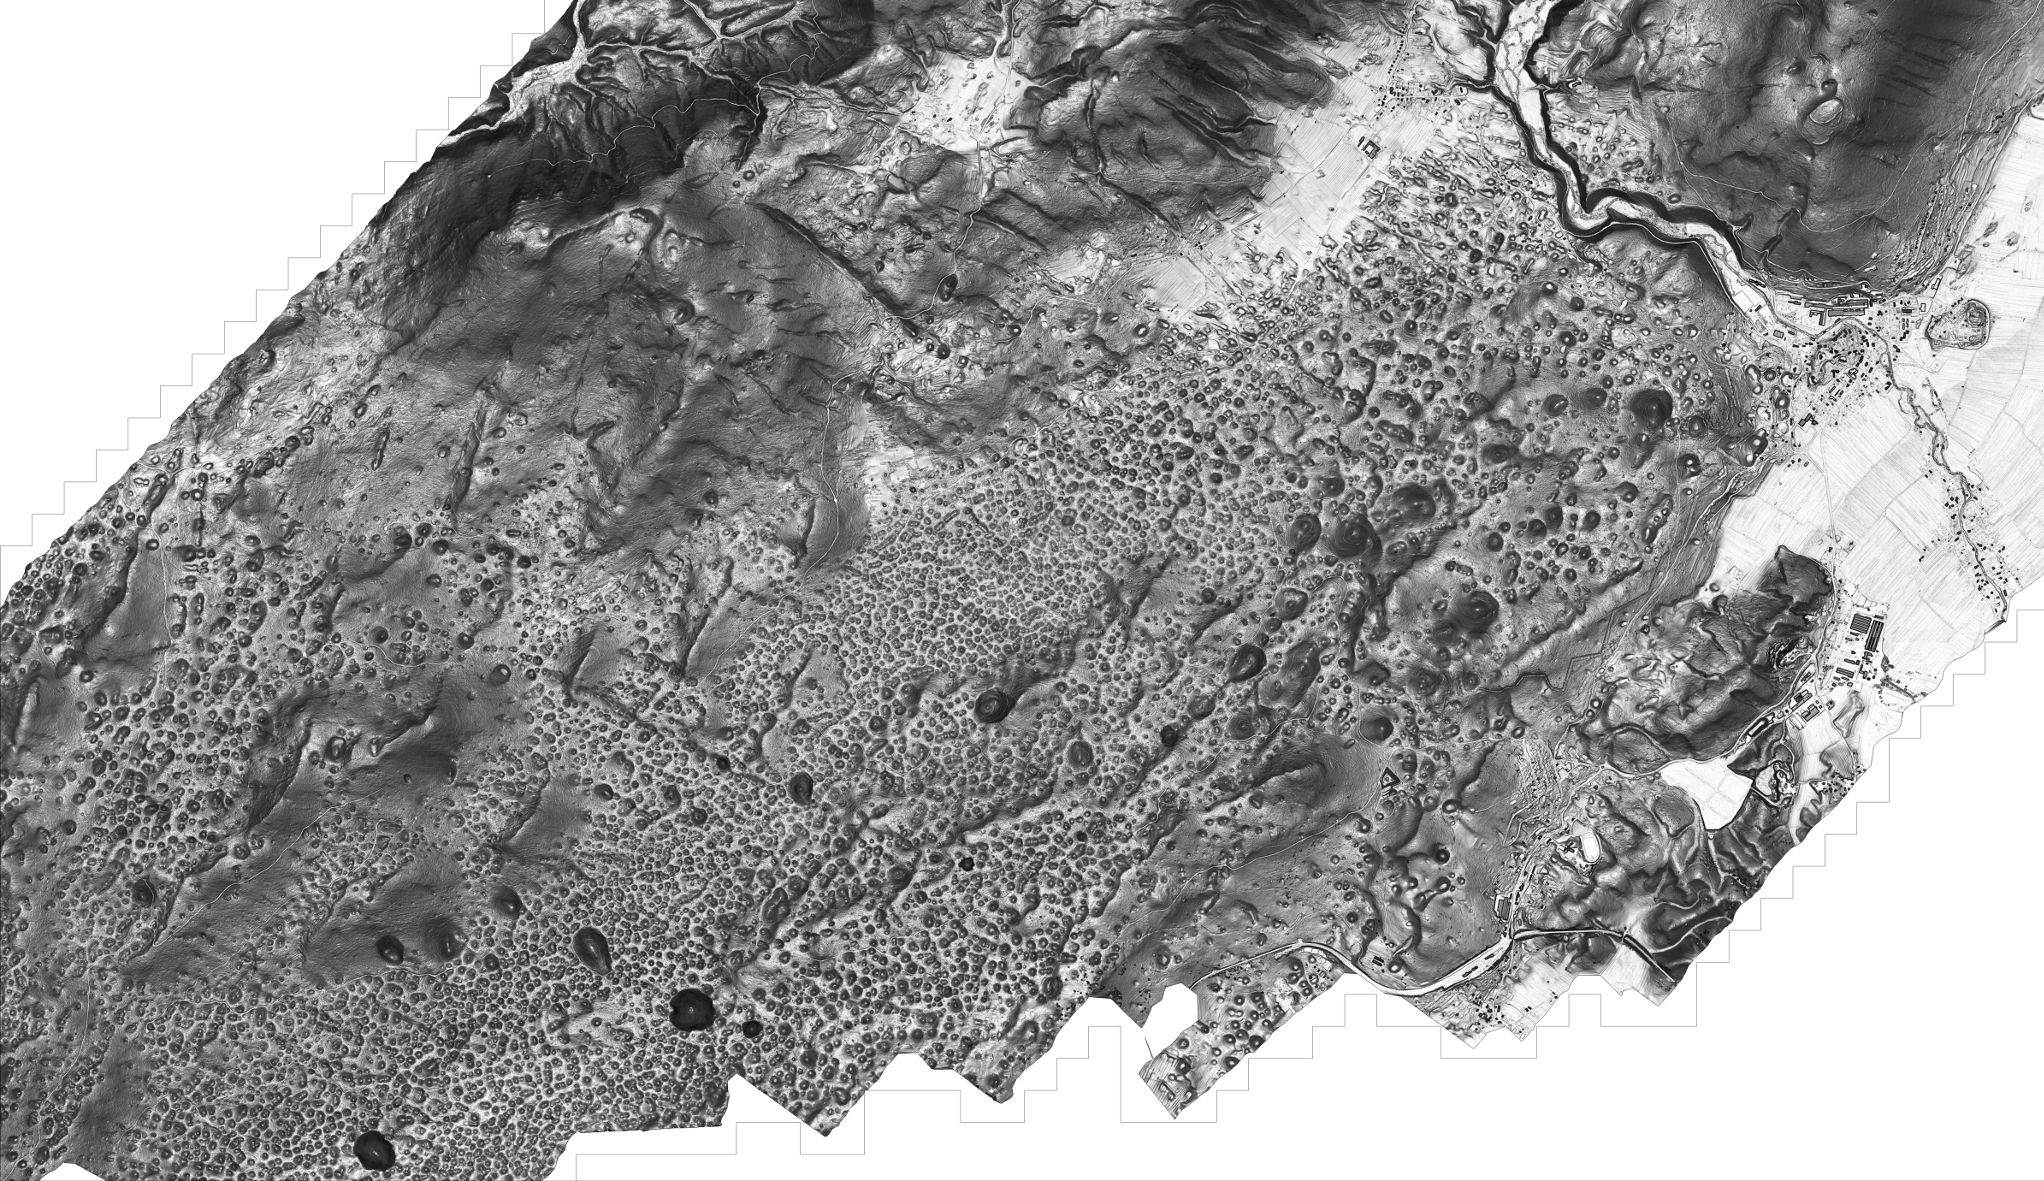
\includegraphics[width=11cm]{slike/menisija-relief.png}
  \caption{Menišija, območje med Cerknico in Logatcem vsebuje nekaj tisoč vrtač in več udornic}
  \label{fig:menisija-relief}
\end{figure}

\begin{figure}
  \begin{center}
    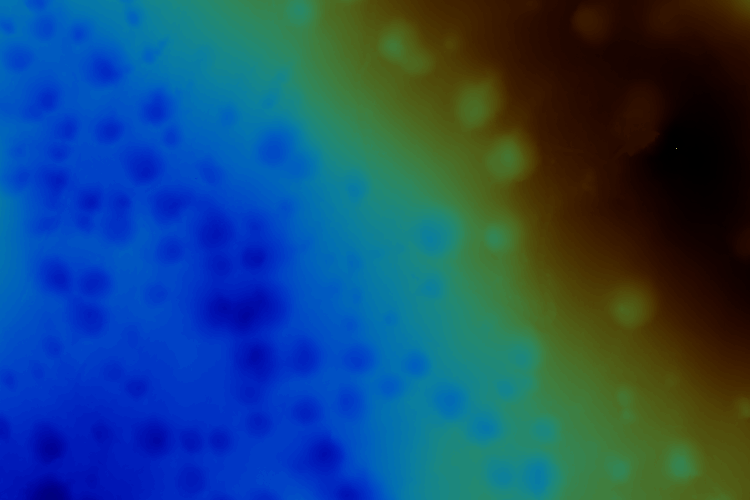
\includegraphics[width=9cm]{slike/D22-35-10}
  \end{center}
  \caption{Relief D22-35-10}
  \label{pic1}
\end{figure}

\begin{figure}
  \begin{center}
    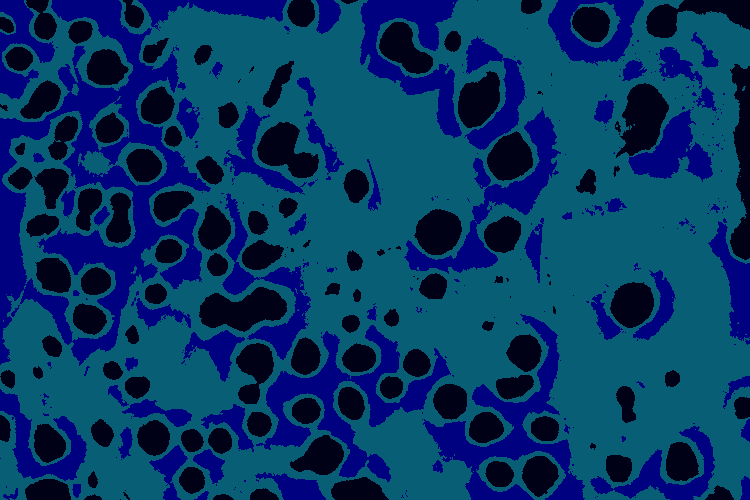
\includegraphics[width=9cm]{slike/D22-35-10-TPI}
  \end{center}
  \caption{Topology Position Index reliefa D22-35-10}
  \label{pic2}
\end{figure}

\begin{figure}
  \begin{center}
    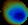
\includegraphics[width=3cm]{slike/D22-35-10-fig11}
    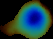
\includegraphics[width=3cm]{slike/D22-35-10-fig14}
    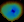
\includegraphics[width=3cm]{slike/D22-35-10-fig32}
  \end{center}
  \caption{Primer vrtač iz reliefa D22-35-10}
  \label{pic3}
\end{figure}

\chapter{Numerično modeliranje skupine vrtač}
\label{ch2}

\section{Stohastične korozijske točke}
\section{Semistohastične polzeče korozijske točke}
\section{Preizkus modela korozijskih točk na geološki karti}


%\chapter{}

\chapter{Analitično modeliranje posamezne vrtače}
\label{ch3}

\section{Elastomehanični model}
\section{Boussinesqov približek}


%%%%%%%%%%%%%%%%%%%%%%%%%%%%%%%%%%%%%%%%
%\begin{comment}
%%%%%%%%%%%%%%%%%%%%%%%%%%%%%%%%%%%%%%%%

\chapter{Zaključek}


%%%%%%%%%%%%%%%%%%%%%%%%%%%%%%%%%%%%%%%%
%\end{comment}
%%%%%%%%%%%%%%%%%%%%%%%%%%%%%%%%%%%%%%%%

\nocite{*}
\newpage
\bibliography{bibliography}{}
\bibliographystyle{alpha}


\end{document}

